\documentclass{standalone}
\usepackage{tikz}
\usetikzlibrary{positioning}
\usetikzlibrary{calc}
\def\mainpath{../../}
\def\tikzpath{./}
\usepackage{pgfplots}
\usepackage{pgfplotstable}
\usetikzlibrary{pgfplots.groupplots}
\usepackage{import}


\definecolor{list1_1}{RGB}{0,101,189}
\definecolor{list1_2}{RGB}{156,157,159}
\definecolor{list1_3}{RGB}{162,173,0}
\definecolor{list1_4}{RGB}{227,114,34} 
\definecolor{list1_5}{RGB}{152,198,234}


%\definecolor{list1_1}{RGB}{246,81,29}
%\definecolor{list1_2}{RGB}{255,180,0}
%\definecolor{list1_3}{RGB}{0,166,237}
%\definecolor{list1_4}{RGB}{127,184,0}
%\definecolor{list1_5}{RGB}{13,44,84}


\pgfplotscreateplotcyclelist{markerlist}{
list1_1, thick, solid, mark=*\\%
list1_2, thick, solid, mark=asterisk\\%
list1_3, thick, solid, mark=diamond*\\%
list1_4, thick, solid, mark=triangle\\%
list1_5, thick, solid, mark=square\\%
}

\pgfplotscreateplotcyclelist{linelist}{
list1_1, solid\\%
list1_2, solid\\%
list1_3, solid\\%
list1_4, solid\\%
list1_5, solid\\%
}

\definecolor{lightgrey}{RGB}{200,200,200}
\definecolor{nassitextcolor}{RGB}{0,0,200}
\begin{document}
\begin{tikzpicture}
	\def\subsize{2}%
	   \def\sep{1.0}    %separation between rectangles       
       %define nodes
       \node (N1) at (-\subsize,-\subsize)  {};%{N1};
       \node (N2) at (0        ,-\subsize)  {};%{N1};
       \node (N3) at (+\subsize,-\subsize)  {};%{N1};
       \node (N4) at (-\subsize,0)          {};%{N1};
       \node (N5) at (0        ,0)          {};%{N1};
       \node (N6) at (+\subsize,0)          {};%{N1};
       \node (N7) at (-\subsize,\subsize)   {};%{N1};
       \node (N8) at (0        ,\subsize)   {};%{N1};
       \node (N9) at (+\subsize,\subsize)   {};%{N1};
       
               % nodes
       \node (N11) at (-\sep-\subsize,+\sep)          {};%{N11};
       
       \node (N12) at (-\sep         ,+\sep)          {};%{N12};
       \node (N13) at (-\sep         ,+\sep+\subsize) {};%{N13};
       \node (N14) at (-\sep-\subsize,+\sep+\subsize) {};%{N14};
       
       \node (N21) at (+\sep         ,+\sep          ){};%{N21};
       \node (N22) at (+\sep+\subsize,+\sep          ){};%{N22};
       \node (N23) at (+\sep+\subsize,+\sep+\subsize) {};%{N23};
       \node (N24) at (+\sep         ,+\sep+\subsize) {};%{N24};
       
       \node (N31) at (+\sep,-\sep-\subsize)          {};%{N31};
       \node (N32) at (+\sep+\subsize,-\sep-\subsize) {};%{N32};
       \node (N33) at (+\sep+\subsize,-\sep)          {};%{N33};
       \node (N34) at (+\sep,-\sep)                   {};%{N34};
       
       \node (N41) at (-\sep-\subsize,-\sep-\subsize) {};%{N41};
       \node (N42) at (-\sep,-\sep-\subsize)          {};%{N42};
       \node (N43) at (-\sep,-\sep)                   {};%{N43};
       \node (N44) at (-\sep-\subsize,-\sep)          {};%{N44};
	%\subimport{./}{setup_quad4_basic_example_nodes.tex}
	\end{tikzpicture}
		\begin{tikzpicture}
				\def\subsize{2}%
		\def\sep{1.0}    %separation between rectangles
				\draw[fill=lightgrey,thick] (N31) rectangle (N33);
		    \node[anchor=south west]  at (N31) {$\mathit{_{2}^{1}}$};%{N31};
            \node[anchor=south east]  at (N32) {$\mathit{_{4}^{3}}$};%{N32};
            \node[anchor=north east]  at (N33) {$\mathit{_{8}^{7}}$};%{N33};
            \node[anchor=north west]  at (N34) {$\mathit{_{6}^{5}}$};%{N34};
            
                   %lagrange multipliers
       \draw[->] (N12) edge (N34) node [fill=white, font=\small] at ($(N12)!0.35!(N34)$) {\framebox{$_6^5$}};
       \draw[->] (N21) edge (N34) node [fill=white, font=\small] at ($(N21)!0.5!(N34)$) {\framebox{$_{12}^{11}$}};
       \draw[->] (N22) edge (N33) node [fill=white, font=\small] at ($(N22)!0.5!(N33)$) {\framebox{$_{14}^{13}$}};
       \draw[<-] (N31) edge (N42) node [fill=white, font=\small] at ($(N31)!0.5!(N42)$) {\framebox{$_{18}^{17}$}};   
       \draw[<-] (N34) edge (N43) node [fill=white, font=\small] at ($(N34)!0.5!(N43)$) {\framebox{$_{20}^{19}$}};
       
       %\node at (N41) {};
       %\node at (-5,0) {};
				
				
		\end{tikzpicture}
		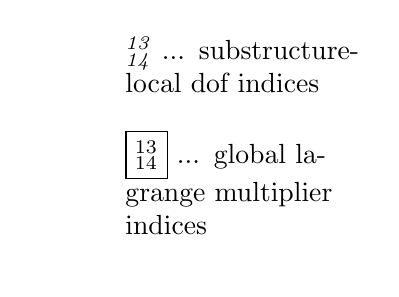
\begin{tikzpicture}
		\node [anchor=south west,text width=3cm, node distance=1.5cm] (I11) at (1,0) {$\mathit{_{14}^{13}}$ ... substructure-local dof indices};
		\node [anchor=south west,below of = I11,text width=3cm, node distance=1.5cm] (I2) {\framebox{$_{14}^{13}$} ... global lagrange multiplier indices\\};
		\node at (0,-2) {};
		\end{tikzpicture}
\end{document}